\newpage
\section{Extending MetaDoc}
\label{sec:extending}
To extend MetaDoc to send more data, the following is needed. Each step is 
explained in more detail below. Certain restrictions is set on how the XML
document should be formed. See section \ref{sec:xmldoc} for more information.

\begin{itemize}
    \item
        Definition of data to be sent in the MetaDoc DTD.
    \item
        A definition file explaining the data on the client.
    \item
        An entries file, explaining any entries allowed in the data on the 
        client.
    \item
        A \texttt{MetaInput} or \texttt{MetaOutput} sub-class that should
        handle data, depending on whether data is recieved or sent to or from
        the server, respectively.
    \item
        Adding a handle to \texttt{main.py} that will activate the data type.
    \item
        Configuring the server to send or recieve the intended data.
\end{itemize}

Figure \ref{fig:connection_example} shows an example of how the data for
projects is defined, and the connection between classes that are used when data
about projects is recieved from the server.

\begin{figure}[h!]
    \includegraphics[width=\textwidth]{img/example}
    \caption{Example of how projects data is defined and connection between
    classes used in definition and processing of project data.}
    \label{fig:connection_example}
\end{figure}

\subsection{Altering DTD}
\textit{The XML document follows certain conventions that should be followed when
extending the DTD. These conventions are explained in more detail in section
\ref{sec:xmldoc}.}

Before you alter the DTD you should know exactly what data should be sent.
Create an \texttt{<!ELEMENT>} with a descriptive name of the data sent. As an
example, \texttt{<users>} is used for a list of users. 

Add any attributes necessary to describe the set of data. If the data is a list
of entries, such as a list of users, create an \texttt{<!ELEMENT>} as a
possible sub-element that contains the information about each entry. Any short
information about the entry should be placed in attributes of the entry. If
there is more information, such as information that could be several sentences
or lines, it should not be placed as an attribute. This information should be
placed inside the element itself. If there are several types of long
information for each entry, create a descriptive \texttt{<!ELEMENT>} for each
as a sub-element of each entry to contain the text. Otherwise the text may be
placed directly inside the entry element itself. 

\subsection{Defining the data on the client}
\label{sec:defclientmodel}
Add a module to the client with the name of the main element. Create a file
\texttt{definition.py} inside this module. \texttt{definition.py} should define
the main element with a subclass of \texttt{metaelement.MetaElement}.

Create a file \texttt{entries.py} inside the same module. This file should
contain definitions of each entry, and potential sub-elements for each entry,
as a sub-class of \texttt{metaelement.MetaElement}. 

Add the entry class(es) to \texttt{self.legal\_element\_types} of the \\ 
\texttt{metaelement.MetaElement} sub-class defining the main element. 

\texttt{metaelement.MetaElement} sub-classes may define a
\texttt{clean\_<attribute name>()} for each attribute on the element. This method
will recieve the attribute value, and should return the attribute value after
any potential cleaning is done on it. Please note that \textit{all} attribute
values \textit{must} be strings, so if any value set as an attribute might be
set as anything other than a string, the clean-function is the place to convert
it.

\subsection{Custom client handles}
If the data is to be sent from client to server, create a module
\texttt{custom/site<main element name>.py} that contains a sub-class of
\texttt{custom.abstract.MetaOutput}. This class should define a method
\texttt{populate()} which gathers the information to be sent from the site and
appends an instance of a entry-class, as defined in section
\ref{sec:defclientmodel}, to \texttt{self.items} for each entry.

\subsection{Versioning}
MetaDoc passes a \textbf{version} attribute on it's root element,
\texttt{<MetaDoc>} when sending information between client and server. This
version is a number on the form ''\texttt{X}.\texttt{Y}.\texttt{Z}'', where
\texttt{X}, \texttt{Y} and \texttt{Z} are numbers. Changes made to each number 
indicate different levels of breakage. 

When \texttt{X} is changed, changes are made such that the current information
passed is changed in some way. This may be changes to the DTD where any of the
currently passed information is affected (addition/removal of attributes,
changes to how attribute values are presented or should be parsed,
addition/removal of sub-elements). If the client or server encounters a
document with a different value of \texttt{X} in the version number, it should
\textit{not} accept the data, as it cannot be sure it will handle it correctly.

Changes to \texttt{Y} indicates a change that does \textit{not} change the
current behaviour in any way, but instances where new information might be
passed. When the client or server encounters a document with a different value
of \texttt{Y} it should log a warning, but otherwise proceed as normally.

\texttt{Z} is currently not used for anything, but is present for potential
usability in the future. Differences in \texttt{Z} should be logged as debug
information.
